\begin{frame}{Wie kommt es zu einem Modell?}
    
\begin{block}{Ausgangspunkte}

    \begin{itemize}
        \item Prototyping
        \item Nachbildung von Bauteilen
        \item Nachbildung von kulturellen Gütern
        \item Modell für die Erweiterung oder Nachbearbeitung
    \end{itemize}
    
\begin{figure}[]
    \begin{minipage}{.45\textwidth}
        \begin{figure}[l]
            \centering
            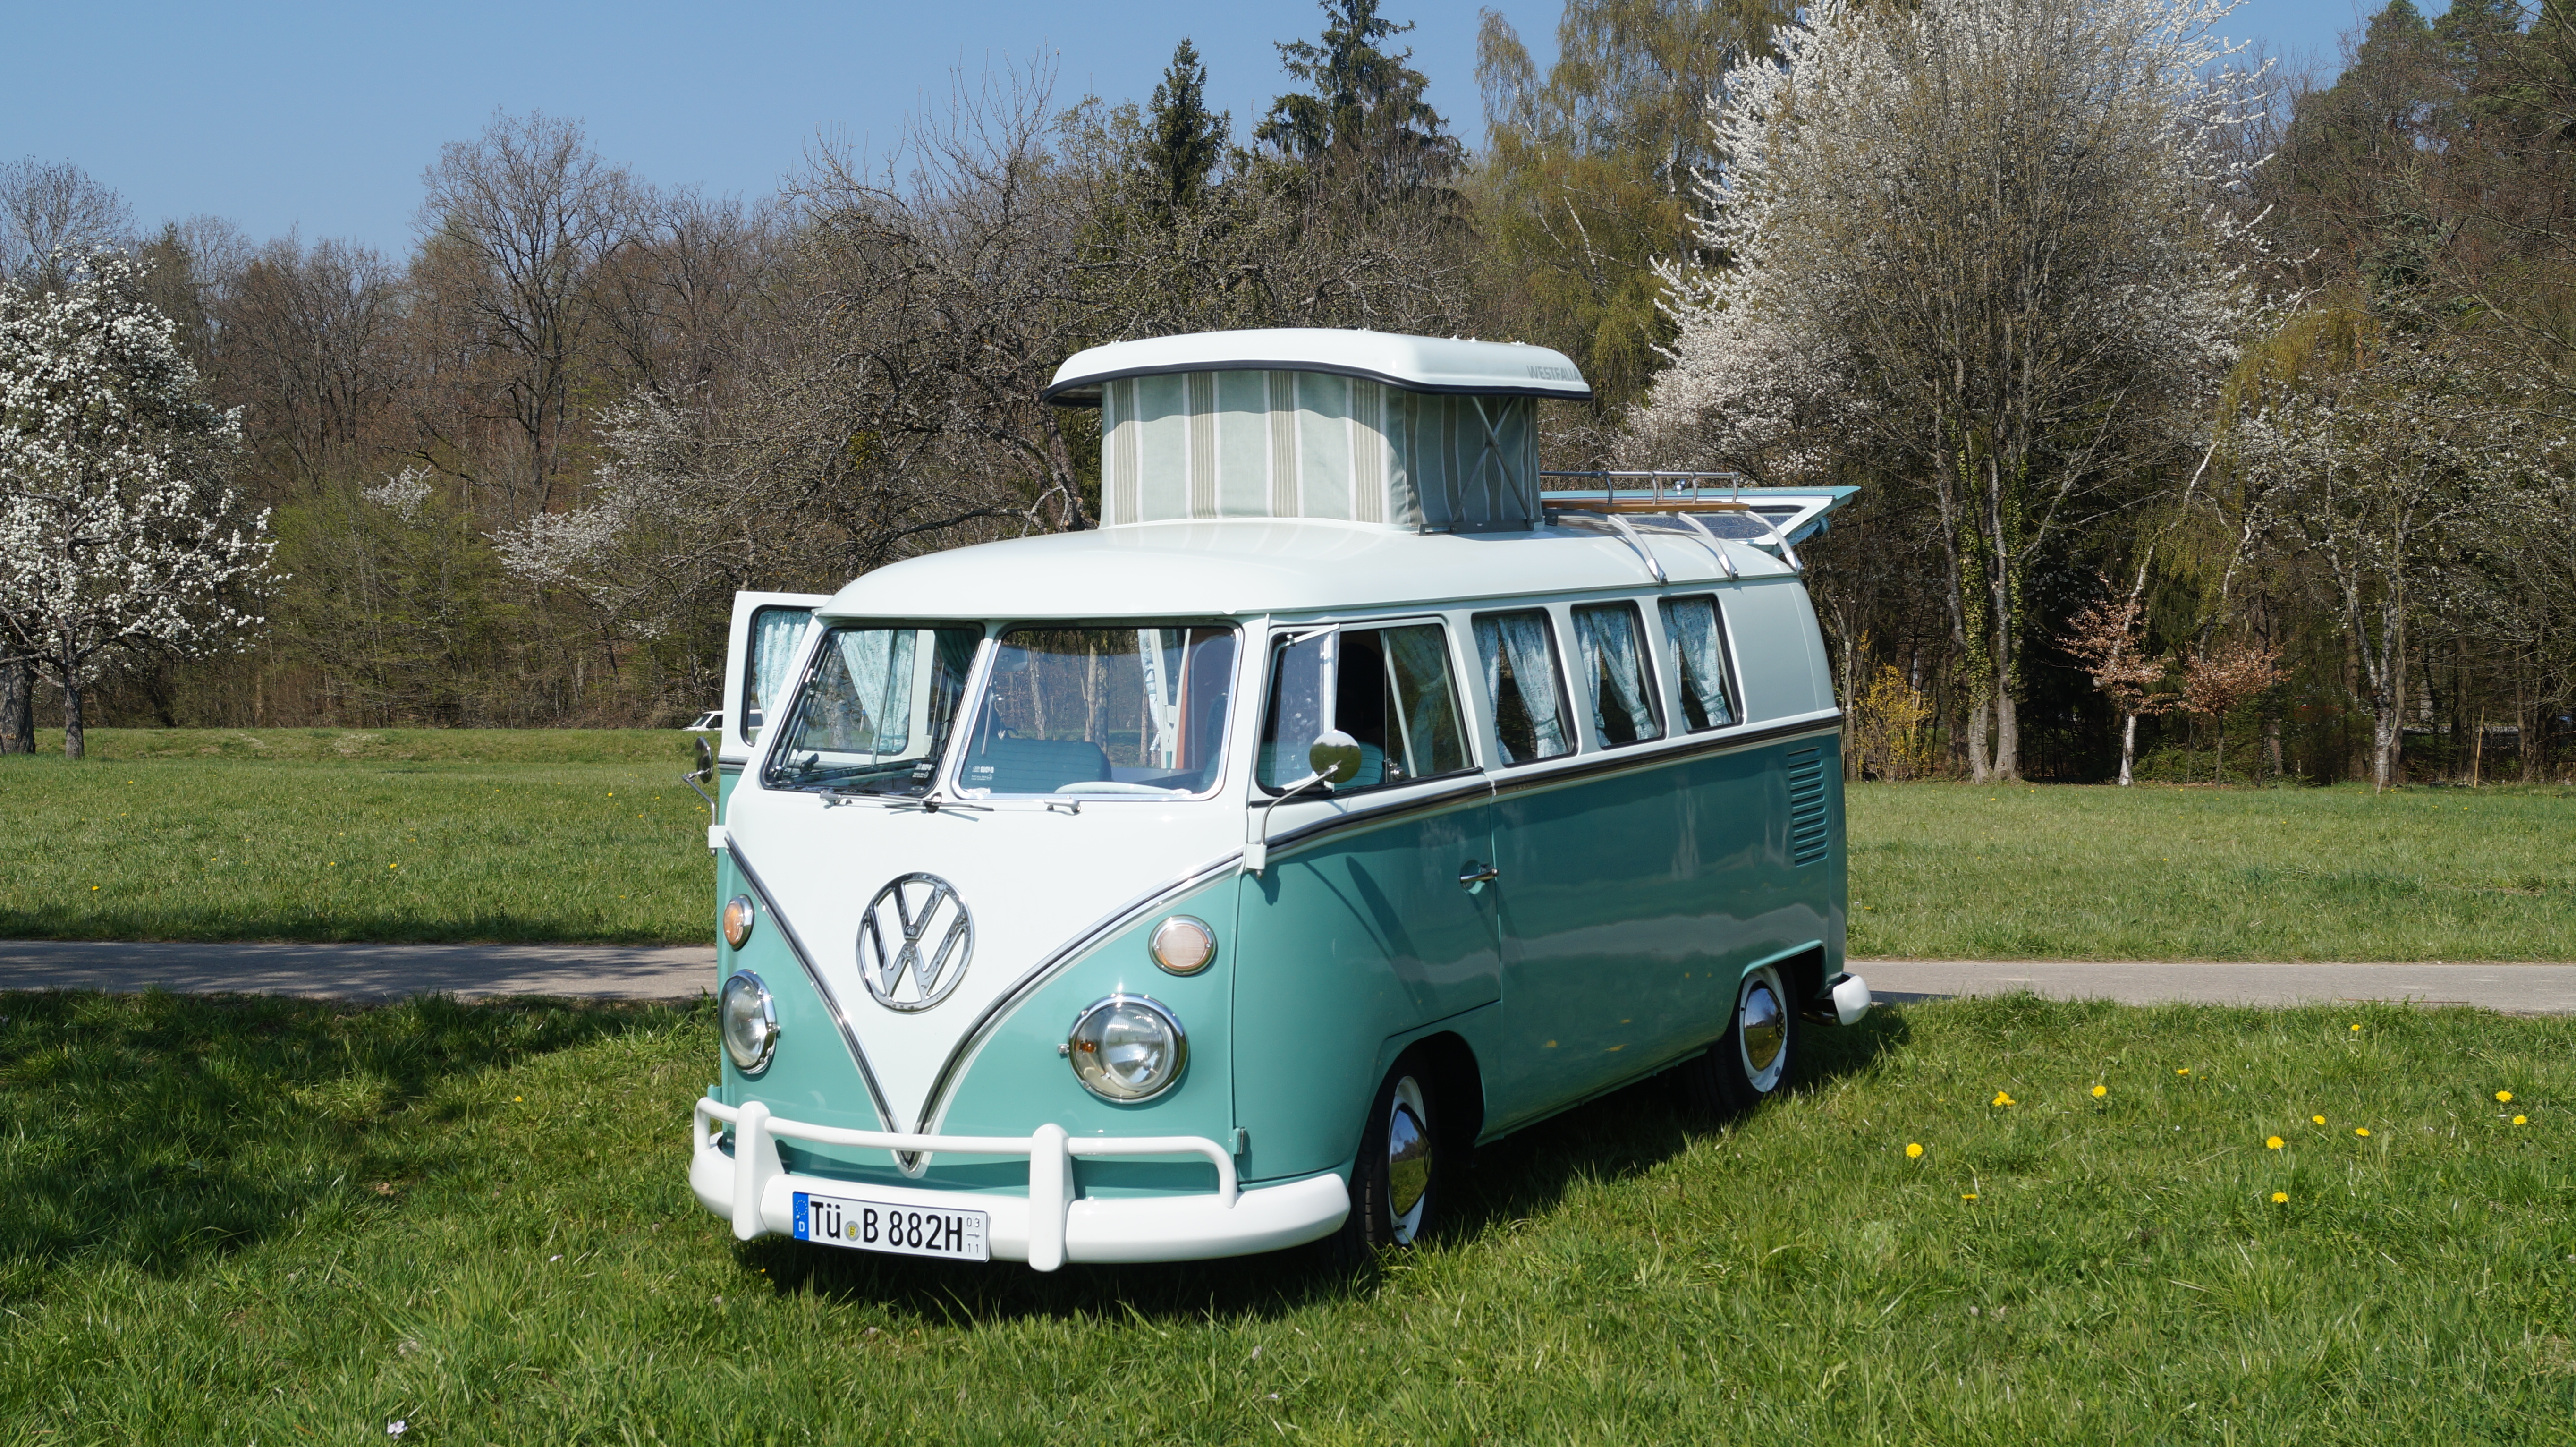
\includegraphics[width=175pt]{img_niklas/flo.JPG}
            \label{fig:my_label}
        \end{figure}
    \end{minipage}
    \hfill
    \begin{minipage}{.45\textwidth}
        \begin{figure}[r]
            \centering
            \includegraphics[width=175pt, angle=180]{img_niklas/ersatzteil2.jpg}
            \label{fig:my_label}
        \end{figure}    
    \end{minipage}
\end{figure}

\end{block}
\end{frame}

\begin{frame}{3D Scanning}
    
    \begin{minipage}[m]{.49\textwidth}
    \begin{block}{Photogrammetrie}
        \begin{itemize}
            \item \textbf{Bilder aus vielen Winkeln}
            \item Ermittlung 3D Koordinaten
            \item Point-Cloud bilden
            \item Mesh Netz spannen
            \item Rechenintensiver Prozess
            \item hohen Leistungsaufwand
            \item Qualität abhängig von Bildern
        \end{itemize}    
    \end{block}
    \end{minipage}
    \begin{minipage}[m]{.49\textwidth}
        \begin{figure}[]
          \includegraphics[width=190pt]{img_niklas/photogrammetrie_6014830.jpg}
          \label{fig:my_label}
      \end{figure}    
    \end{minipage}
    
\end{frame}

\begin{frame}{3D Scanning}
    \begin{minipage}[m]{.49\textwidth}
    \begin{block}{Photogrammetrie}
        \begin{itemize}
            \item Bilder aus vielen Winkeln
            \item \textbf{Ermittlung 3D Koordinaten}
            \item Point-Cloud bilden
            \item Mesh Netz spannen
            \item Rechenintensiver Prozess
            \item hohen Leistungsaufwand
            \item Qualität abhängig von Bildern
        \end{itemize}
        \end{block}
    \end{minipage}
    \begin{minipage}[m]{.49\textwidth}
        \begin{figure}[]
          \includegraphics[height=130pt]{img_niklas/Structure-from-Motion-SfM-process-is-illustrated-The-structure-in-the.png}
          \label{fig:my_label}
      \end{figure}    
    \end{minipage}
    
\end{frame}

\begin{frame}{3D Scanning}
\begin{minipage}[m]{.49\textwidth}
    \begin{block}{Photogrammetrie}
        \begin{itemize}
            \item Bilder aus vielen Winkeln
            \item Ermittlung 3D Koordinaten
            \item \textbf{Point-Cloud bilden}
            \item Mesh Netz spannen
            \item Rechenintensiver Prozess
            \item hohen Leistungsaufwand
            \item Qualität abhängig von Bildern
        \end{itemize}  
    \end{block}
    \end{minipage}
    \begin{minipage}[]{.49\textwidth}
        \begin{figure}[]
          \includegraphics[height=130pt]{img_niklas/image_anlasserPointCloud.PNG}
          \label{fig:my_label}
      \end{figure}    
    \end{minipage}
    
  
\end{frame}

\begin{frame}[m]{3D Scanning}
    \begin{minipage}{.49\textwidth}
    \begin{block}{Photogrammetrie}
        \begin{itemize}
            \item Bilder aus vielen Winkeln
            \item Ermittlung 3D Koordinaten
            \item Point-Cloud bilden
            \item \textbf{Mesh Netz spannen}
            \item Rechenintensiver Prozess
            \item hohen Leistungsaufwand
            \item Qualität abhängig von Bildern
        \end{itemize}
    \end{block}
    \end{minipage}
    \begin{minipage}[m]{.49\textwidth}
        \begin{figure}[]
          \includegraphics[height=130pt]{img_niklas/image_anlasserMesh.PNG}
          \label{fig:my_label}
      \end{figure}    
    \end{minipage}
    
\end{frame}

\begin{frame}[m]{3D Scanning}
    \begin{minipage}{.49\textwidth}
    \begin{block}{Photogrammetrie}
        \begin{itemize}
            \item Bilder aus vielen Winkeln
            \item Ermittlung 3D Koordinaten
            \item Point-Cloud bilden
            \item Mesh Netz spannen
            \item \textbf{Rechenintensiver Prozess}
            \item \textbf{hohen Leistungsaufwand}
            \item Qualität abhängig von Bildern
        \end{itemize}
    \end{block}
    \end{minipage}    
    \begin{minipage}[m]{.49\textwidth}
        \begin{figure}[]
          \includegraphics[height=130pt]{img_niklas/rock_image.PNG}
          \label{fig:my_label}
      \end{figure}    
    \end{minipage}
    
\end{frame}


\begin{frame}{3D Scanning}
    
    \begin{minipage}[m]{.49\textwidth}
    \begin{block}{Photogrammetrie}
        \begin{itemize}
            \item Bilder aus vielen Winkeln
            \item Ermittlung 3D Koordinaten
            \item Point-Cloud bilden
            \item Mesh Netz spannen
            \item Rechenintensiver Prozess
            \item hohen Leistungsaufwand
            \item \textbf{Qualität abhängig von Bildern}
        \end{itemize}   
    \end{block}
    \end{minipage}
    \begin{minipage}[m]{.49\textwidth}
        \begin{figure}[]
          \includegraphics[height=130pt]{img_niklas/rock_3dscan.PNG}
          \label{fig:my_label}
      \end{figure}    
    \end{minipage}
    
\end{frame}

\begin{frame}{3D Scanning}
    \begin{block}{Laserscanning}
     \begin{figure}[t]
        \centering
        \begin{minipage}[m]{0.3\textwidth}
        \begin{figure}
            \centering
            \includegraphics[height=60pt]{img_niklas/shining-3d-einscan-hx-software-bundle-solid-edge-essentials-1-stk-338985-de.png}
            \label{fig:my_label}
        \end{figure}
        \begin{figure}[b]
            \centering
            \includegraphics[height=90pt]{img_niklas/3d-scanning-101_9.jpg}
            \label{fig:my_label}
        \end{figure}
        \end{minipage}
        \hfill
        \begin{minipage}[m]{0.3\textwidth}
         \begin{figure}
            \centering
            \includegraphics[height=60pt]{img_niklas/3dprintingaHouse.PNG}
            \label{fig:my_label}
        \end{figure}
        \begin{figure}[b]
            \centering
            \includegraphics[height=80pt]{img_niklas/3dprintingaHouse2.PNG}
            \label{fig:my_label}
        \end{figure}
        \end{minipage}
        \hfill
        \begin{minipage}[m]{0.3\textwidth}
            \begin{itemize}
                \item Alternative zu Fotos
                \item Genaueres Ergebnis
                \item Schlechter skalierbar
                \item Teure Anschaffung
                \item Nicht immer möglich
                \item Usecase abhängig
            \end{itemize}
        \end{minipage}
    \end{figure}
    \end{block}
\end{frame}

\begin{frame}{Contact 3D scanners}
\begin{figure}
    \centering
    \includegraphics[width=300pt]{img_niklas/CMM.png}
    \caption*{Coordinate measuring machine}
    \label{fig:my_label}
\end{figure}
    
\end{frame}

